\section{Poisons}
Athasian bards are masters of the dark art of poisoning, and of the fine art of creating potent poisons out of plant extracts and creature venom.

\begin{figure*}[b!]
\centering
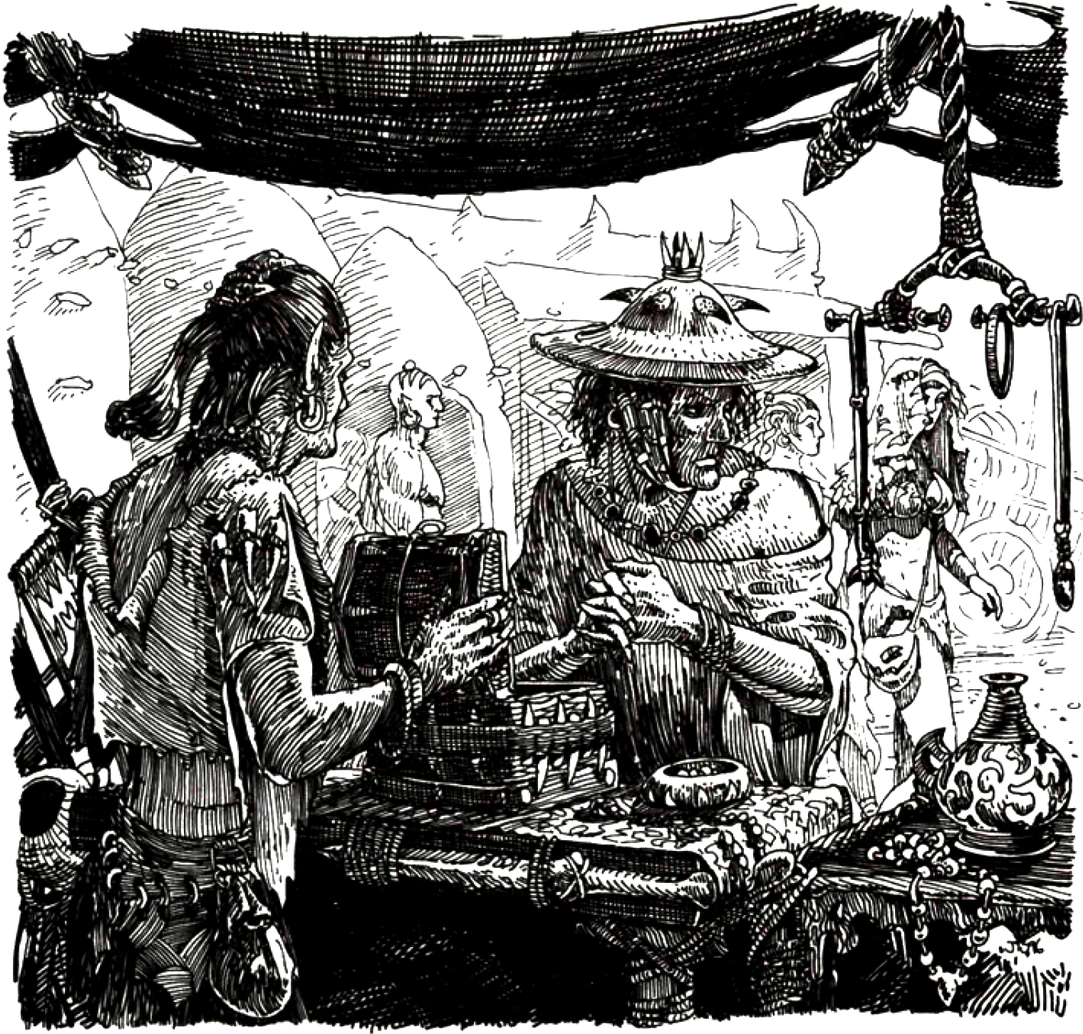
\includegraphics[height=0.4\paperheight]{images/merchant-2.png}
\par\textit{\small\textcopyright Wizards of the Coast, 2020.}
\end{figure*}

\BigTablePair{Non-Injury Poisons}{l l X X r{11mm}}{
\tableheader Name & \tableheader Save DC & \tableheader Initial Damage & \tableheader Secondary Damage & \tableheader Price\\

\multicolumn{5}{l}{\TableSubheader{Contact}}\\
Mulworm & DC 10 & 2d6 Dex & 1d6 Con & 120 cp\\
Beetle, dragon\footnotemark[1] & DC 12 & 2d6 Con & 2d6 Con & 150 cp\\
Sassone leaf residue & DC 16 & 2d12 hp & 1d6 Con & 300 cp\\
T'liz essence & DC 16 & $\star$ & --- & 400 cp\\
T'chowb ichor & DC 13 & 1 Int$^\dagger$ & 2d4 Int + 1 Int$^\dagger$ & 500 cp\\
Malyss root paste & DC 16 & 1 Dex & 2d4 Dex & 500 cp\\
Nitharit & DC 13 & --- & 3d6 Con & 650 cp\\
Id fiend essence & DC 16 & shaken 1 minute & panicked 2d6 minutes & 750 cp\\
Terinav root & DC 16 & 1d6 Dex & 2d6 Dex & 750 cp\\
Dragon bile & DC 26 & 3d6 Str & --- & 1,500 cp\\
Antloid, soldier (contact) & DC 16 & 2d6 Con & --- & 1,800 cp\\
Black lotus extract & DC 20 & 3d6 Con & 3d6 Con & 4,500 cp\\

\multicolumn{5}{l}{\TableSubheader{Ingested}}\\
Kivit & DC 10 & 1d3 Con & 1d3 Con & 90 cp\\
Oil of taggit & DC 15 & --- & Unconsciousness & 90 cp\\
Arsenic & DC 13 & 1 Con & 1d8 Con & 120 cp\\
Id moss & DC 14 & 1d4 Int & 2d6 Int & 125 cp\\
Kank taint\footnotemark[2] & DC 13 & 1d4 Con + $\star$ & --- & 125 cp\\
Mulworm & DC 12 & 1d6 Con & 1d6 Con & 125 cp\\
Crescent forest wine & DC 16 & 1d3 Int & 1d4 Int +1d3 Str & 175 cp\\
Striped toadstool & DC 11 & 1 Wis & 2d6 Wis + 1d4 Int & 180 cp\\
Lich dust & DC 17 & 2d6 Str & 1d6 Str & 250 cp\\
Dark reaver powder & DC 18 & 2d6 Con & 1d6 Con + 1d6 Str & 300 cp\\
Elf scent & DC 16 & skill penalty & --- & 300 cp\\
Purple grass extract & DC 15 & 4d10 hit points & $\star$ & 500 cp\\
Bleached inix slumber & DC 16 & $\star$ & $\star$ & 650 cp\\
Fael appetite & DC 14 & 1d6 Wis + $\star$ & 1d6 Wis + $\star$ & 700 cp\\
Methelinoc & DC 16 & 1d6 Con & 1d6 Con & 800 cp\\
Zombie plant extract & DC 15 & 1d6 Int & 2d6 Int + $\star$ & 1,300 cp\\
Fruit, tree of death\footnotemark[3] & DC 22 & 4d6 Con & 4d6 Con & 4,500 cp\\
Templar's ultimatum & DC 23 & suggestibility 1 minute & 5d6 Con & 5,000 cp\\

\multicolumn{5}{l}{\TableSubheader{Inhaled}}\\
Ungol dust & DC 15 & 1 Cha & 1d6 Cha + 1 Cha$^\dagger$ & 1,000 cp\\
Brain seed powder & DC 14 & 1d4 Wis & 2d4 Wis & 1,100 cp\\
Gaj poison gas & DC 16 & 1d4 Con and nauseated for 1 round & --- & 1,200 cp\\
Insanity mist & DC 15 & 1d4 Wis & 2d6 Wis & 1,500 cp\\
Burnt othur fumes & DC 18 & 1 Con1 & 3d6 Con & 2,100 cp\\
Jalath'gak & DC 16 & paralysis 2d6 rounds & --- & 3,000 cp\\
Fordorran & DC 16 & 2d6 Dex & 3d6 Dex & 3,500 cp\\
Jalath'gak, giant & DC 21 & paralysis 3d6 rounds & --- & 4,500 cp\\
Poisonweed spores & DC 21 & unconsciousness 2d6 minutes & unconsciousness 2d6 minutes & 6,500 cp\\

% \TableNote[p{\columnwidth}]{5}{vish}\\
\BigTableNote{5}{$\star$ See entry.}\\
\BigTableNote{5}{$\dagger$ Permanent drain, not temporary damage.}\\
\BigTableNote{5}{1 Only affects dray and creatures with the Dragon type.}\\
\BigTableNote{5}{2 Affects creatures with the Elemental type, and creatures with the air, earth, fire, and/or water subtype---including those that are otherwise immune to poison.}\\
\BigTableNote{5}{3 Cannot be crafted.}\\
}

\BigTablePair{Injury Poisons}{l l X X r{11mm}}{
\tableheader Name & \tableheader Save DC & \tableheader Initial Damage & \tableheader Secondary Damage & \tableheader Price\\

% \multicolumn{6}{l}{\textit{Injury}}\\
Cactus, spider & DC 12 & paralysis for 2d4 rounds & --- & 75 cp\\
Elven poison & DC 13 & Unconsciousness & Unconsciousness for 2d4 hours & 75 cp\\
Hej-kin & DC 11 & 1 Con & 1 Con & 80 cp\\
Assassin bug & DC 10 & 1d3 Dex & 1d3 Dex & 90 cp\\
Blight & DC 10 & paralysis & paralysis & 90 cp\\
Small centipede poison & DC 11 & 1d2 Dex & 1d2 Dex & 90 cp\\
Bloodroot & DC 12 & --- & 1d4 Con + 1d3 Wis & 100 cp\\
Dust glider & DC 13 & 1d4 Str & 1d4 Str & 100 cp\\
Greenblood oil & DC 13 & 1 Con & 1d2 Con & 100 cp\\
Wall walker & DC 14 & paralysis 1d6 rounds & --- & 100 cp\\
Dune freak & DC 14 & 1 point Str & 1d6 Str & 110 cp\\
Silt serpent & DC 10 & 1d6 Str & 1d6 Con & 110 cp\\
Spider, dark defiler & DC 13 & 1d6 Con & --- & 110 cp\\
Black adder venom & DC 11 & 1d6 Con & 1d6 Con & 120 cp\\
Blue whinnis & DC 14 & 1 Con & Unconsciousness & 120 cp\\
Kank, soldier & DC 13 & 1d6 Str & 1d6 Str & 120 cp\\
Scorpion, gold & DC 12 & 1d6 Str & 1d4 Str & 120 cp\\
Thri-kreen & DC 11 & paralysis & paralysis & 120 cp\\
Pulp bee & DC 14 & 1d4 Dex & 1d4 Dex & 130 cp\\
Spider, dark psion & DC 14 & 1d6 Con & --- & 130 cp\\
Boneclaw, lesser & DC 10 & 1d6 Con & 1d6 Con & 150 cp\\
Floater & DC 13 & paralysis & --- & 150 cp\\
Jankx & DC 11 & 1d6 Str & 2d6 Dex & 150 cp\\
Medium spider venom & DC 14 & 1d4 Str & 1d4 Str & 150 cp\\
Trin & DC 13 & paralysis & paralysis & 150 cp\\
Spider, dark warrior & DC 15 & 1d6 Con & --- & 175 cp\\
Silt horror, black & DC 14 & paralysis for 1 minute & paralysis 1d6 rounds & 180 cp\\
Spider, silt & DC 13 & paralysis & paralysis & 180 cp\\
Wezer, soldier & DC 13 & unconsciousness 1 minute & unconsciousness 2d4 days & 180 cp\\
Braxat hide & DC 18 & --- & $\star$ & 200 cp\\
Cactus, hunting & DC 14 & paralysis 1 minute & paralysis for 1d4+2 rounds & 200 cp\\
Large spider venom & DC 18 & 1d6 Str & 1d6 Str & 200 cp\\
Psionocus & DC 13 & sleep 1 min plus drain PP & sleep 5d6 min plus drain PP & 200 cp\\
Giant wasp poison & DC 18 & 1d6 Dex & 1d6 Dex & 210 cp\\
Mulworm & DC 12 & 1d6 Con & 1d6 Con & 250 cp\\
Shadow essence & DC 17 & 1 Str$^\dagger$ & 2d6 Str & 250 cp\\
Cha'thrang & DC 18 & 1 Str & 2d6 Str & 300 cp\\
Random displays & DC 16 & 1d4 Int & $\star$ & 300 cp\\
Bloodgrass (plains) & DC 13 & 1d6 Dex & paralysis 2d6 rounds & 350 cp\\
Silt serpent, giant & DC 13 & 2d4 Str & 2d4 Con & 375 cp\\
Single-mindedness & DC 15 & 1d4 Wis + $\star$ & --- & 450 cp\\
Halfling tar & DC 17 & unconsciousness & --- & 500 cp\\
Silt serpent, giant (immature) & DC 15 & 2d4 Str & 2d4 Con & 500 cp\\
Purple worm poison & DC 24 & 1d6 Str & 2d6 Str & 700 cp\\
Scorpion, barbed & DC 17 & 1d4 Con & 1d4 Con & 800 cp\\
Blossomkiller & DC 17 & 1d6 Dex & unconsciousness 2d10 minutes & 1,000 cp\\
Silt horror, red & DC 17 & paralysis 2d6 rounds & paralysis 2d6 rounds & 1,000 cp\\
Spider, crystal & DC 17 & 1d6 Con & 1d6 Con & 1,000 cp\\
Mastyrial, desert & DC 18 & 1d6 Con & 1d6 Con & 1,200 cp\\
Mastyrial, black & DC 16 & 2d6 Dex & 1d6 Str & 1,300 cp\\
Spider, mountain & DC 15 & paralysis 2d12 minutes & paralysis 2d12 minutes & 1,350 cp\\
Zik-trin'ak & DC 17 & paralysis & paralysis & 1,350 cp\\
Zik-trin'ta & DC 15 & paralysis & 2d6 Con & 1,500 cp\\
Antloid, soldier (injury) & DC 16 & 2d6 Con & --- & 1,500 cp\\
Scarlet warden & DC 21 & 1d6 Con & 1d6 Con & 1,500 cp\\
Cistern fiend & DC 25 & 1d6 Dex & 2d6 Dex & 1,500 cp\\
Deathblade & DC 20 & 1d6 Con & 2d6 Con & 1,800 cp\\
Bloodgrass (jungle) & DC 19 & 1d6 Dex & paralysis 2d6 rounds & 2,100 cp\\
Spider, dark queen & DC 19 & 1d6 Con & 2d6 Con & 2,100 cp\\
Puddingfish & DC 21 & paralysis 1 minute & paralysis 2d4 rounds & 2,500 cp\\
Silk wyrm & DC 18 & 1d4 Str & paralysis 1d4 days & 2,500 cp\\
S'thag zagath & DC 21 & 1d4 Dex & paralysis 1 minute & 2,500 cp\\
Drik, high & DC 18 & 2d6 Con & 1d6 Con & 2,500 cp\\
Wyvern poison & DC 17 & 2d6 Con & 2d6 Con & 3,000 cp\\
% Drakesblood 3 & DC 25 & 1 point of DR 4 & 1d3 points of DR 4 & 1,500 cp\\

\BigTableNote{5}{$\star$ See entry.}\\
\BigTableNote{5}{$\dagger$ Permanent drain, not temporary damage.}\\
}
Here is the format for poison entries (given as column headings on \tabref{Non-Injury Poisons} and \tabref{Injury Poisons}, below).

\textbf{Type:} The poison's method of delivery---ingested, inhaled, via an injury, or contact

\textbf{Save DC:} The Fortitude save DC needed to avoid the poison's damage.

\textbf{Initial Damage:} The damage the character takes immediately upon failing his saving throw against this type of poison. Ability score damage is temporary unless marked with a dagger ($\dagger$), in which case the loss is a permanent drain instead of temporary damage. Paralysis lasts for 2d6 minutes unless otherwise noted. Unconsciousness lasts for 1d3 hours unless otherwise noted.

\textbf{Secondary Damage:} The amount of damage the character takes 1 minute after exposure as a result of the poisoning, if he fails a second saving throw. Special conditions caused by specific poisons are described below. Effects marked with an asterisk are permanent drain instead of temporary damage.

\textbf{Price:} The price of one dose (one vial) of the poison. It is not possible to use or apply poison in any quantity smaller than one dose. Poisons are normally available only in the city-states' Bard's Quarters, which one always enter at his own risk. Poisons are, likewise, normally illegal to possess within the city-states.

\subsection{Poisons Descriptions}
\textbf{Antloid Poison:} The poison of the soldier antloid causes the instant rupturing of any flesh it contacts, resulting in severe, burn-like wounds that are difficult to heal and often leave horrible scars. Despite the difference in delivery methods, the poison from the archer and infantry antloid soldier are identical; a skilled poison crafter may create either an injury or contact poison using the harvested poison glands from either type of antloid.

\textbf{Assassin Bug Poison:} The poison of the male assassin bug causes a flesh-numbing sensation that ends with a stiffness of the victim's limbs.

\textbf{Barbed Scorpion Poison:} The preferred poison of several elven tribes, the barbed scorpion's poison causes stomach cramping and mild to severe muscle twitching. As with other potent neurotoxins, large or repeat doses of this poison can lead to organ failure and death.

\textbf{Black Mastyrial Poison:} Poison extracted from the black mastyrial's tail stinger leeches feeling from the victim, resulting in the loss of strength and coordination from the body part struck. Repeated doses can render a victim completely numb and useless.

\textbf{Black Silt Horror Venom:} This venom temporarily scrambles brain signals destined for the limbs, resulting in uncontrollable, random body movements that effectively paralyze the victim.

\textbf{Bleached Inix Slumber:} Made from mixing sun bleached inix bone and epserweed sap, this poison is typically mixed with spiced wine. This poison is typically used by bards and templars as a preliminary attack before ambushing rival noble houses, templar officials, or Veiled Alliance cells. Those failing their saving throw fall into a deep slumber for 1d6 hours. Those who are successful on their save suffer a $-2$ penalty to attack and initiative rolls for 1d6 hours. Those who make their save must make an additional save. Failure results in the person being unable to use psionics or cast spells for 2d6 hours.

\textbf{Braxat Hide:} This poison, created from powdered braxat hide and mixed with braxat blood, slowly turns a person's skin into dark green hide, much like that of a braxat. Every day the victim must make a Fortitude save or have 15\% of her body change. For every 30\% of her body that changes, the vicitm gains a +1 natural armor bonus and a $-1$ to Charisma. In addition to the change, every day she fails her save, she takes 1d6 Intelligence or 1d6 Dexterity damage, alternating every day. After two weeks the poison has run its course, with the victim totally or partially changed into a monstrous image of her former self. Once the poison has changed a person, only a \spell{restoration}, \spell{limited wish}, \spell{miracle} or \spell{wish} spell, or the \psionic{reality revision} power, will repair the damage.

This poison is prized by nobles, who use it through bards on their enemies, as well as on their gladiators, hoping to gain the benefits of the change and avoid the damaging factors through healers.

\textbf{Blight Poison:} The undead pixie's poison disrupts the central nervous system's ability to communicate between the brain and the muscles, thereby causing paralysis.

\textbf{Bloodgrass Poison:} Poison harvested from either the plains or jungle variety of the bloodgrass plant disrupts signals between the brain and spinal cord, resulting in loss of coordination and possible paralysis.

\textbf{Blossomkiller Poison:} This paralytic toxin floods the brain with sleep-inducing neurotransmitters, causing immediate drowsiness, vertigo and loss of equilibrium. Shortly thereafter the toxin overwhelms the victim, putting them into a state of deep slumber.

\textbf{Brain Seed Powder:} Although rare and difficult to procure, seed-spores produced by the brain seed plant may be ground down and combined with other materials to produce an inhaled poison that makes a victim more susceptible to mental attacks. Those breathing the powder become disoriented, losing their sense of judgment as their mental faculties become impaired.


\textbf{Cha'thrang Poison:} This alkaloid toxin causes the victim to sweat excessively as it works its way through their system, binding to opioid receptors in their brain and as a result causing severe muscle weakness.

\textbf{Cistern Fiend Poison:} The highly toxic fluid secreted from sacs located at the base of this creature's tentacles can be refined into a potent poison that numbs the victim, inhibiting their motor skills and potentially resulting in paralysis.

\textbf{Crescent Wine:} Derived from the venom of a small, vermin-eating snake found in the Crescent Forest, this alcohol-soluble poison is most commonly mixed into wine (hence the name), where its otherwise bitter taste and alcohol-like effects are easily masked. Victims initially feel groggy and light-headed, as if intoxicated, and as the poison continues to take effect their eyes become glazed and some stomach cramping occurs. Repeated doses eventually put the victim into a coma-like stupor, barely able to move, complete with cold sweats and a drastic slowdown of their heartbeat. This poison is most commonly found in the Bard's Quarter of Nibenay, although it can also be purchased in Gulg and from other black market dealers throughout the Ivory Triangle.

\textbf{Crystal Spider Venom:} Notoriously time-consuming and difficult to extract, refined crystal spider venom binds with iron and other metals in the victim's body, damaging bone marrow and causing severe anemia as well as other potentially life-threatening ailments. The most obvious signs of crystal spider poisoning are a paleness of skin, physical weakness, and an overall feeling of fatigue.

\textbf{Dark Spider Venom:} This venom causes an ulcerous wound that ruptures any skin, muscle and organ tissues it comes into contact with. Depending on the severity of the wound and potency of the venom, the effect of this poison can be deadly as well.

\textbf{Desert Mastyrial Poison:} Unlike its cousin the black mastyrial, the poison from a desert mastyrial causes internal hemorrhaging, resulting in painful splotchy bruises appearing all over the victim's skin, body chills, and possible bleeding from bodily orifices.

\textbf{Dragon Beetle Poison:} This 30-centimeter-long beetle is named after the only creatures that are affected by its poison: dragons, drakes and dray. Against affected creatures, the area around a wound containing the poison swells into a red, burning welt. Soon after the poison enters its victim's body, he feels excruciating pain as if burning from the inside-out. Against any other creature, the poison of the dragon beetle is harmless.

% \textbf{Drakesblood:} Just as the elemental drakes came to be bound to Athas, a large quantity of drake blood can be rendered down into a thick, gummy poison capable of ``binding'' elementals and other elementally-aligned creatures to the prime material plane, thereby lowering their resistance to mundane forms of damage. This poison reduces supernatural damage reduction, causing the creature to suffer more damage from weapons that do not bypass their defenses. Unlike other poisons, drakesblood only affects creatures with the elemental type, or those with the air, earth, fire and/or water subtypes; other creatures that are immune to poison are unaffected, as are creatures whose damage reduction is an extraordinary ability (such as the tough skin of a drake, ironically enough). This poison also affects the appropriate creature types, regardless of any innate resistances to poison they may have (such as an elemental's natural immunity to poison). Repeated DR loss from this poison stacks with previous damage, is treated as ability score damage for the purpose of healing, and cannot reduce a creature's damage reduction below 0.\\For example, an elemental with DR 10/-- is hit with a drakesblood-coated weapon that deals a total of 11 damage, causing 1 point of damage to the elemental and thus affecting it with the injury poison; if the damage had been 10 or less the poison would not have affected the target, as per normal poison rules. The elemental fails its Fortitude save against the poison's primary effect, reducing its DR to 9/--. 10 rounds later it again fails its save against the secondary effect, resulting in an additional 1d3 points of DR lost, potentially reducing it as low as DR 6/--.

\textbf{Dune Freak Venom:} Working directly on the victim's muscle tissue, this venom causes dizziness, fatigue, and muscle weakness.

\textbf{Dust Glider Poison:} When removed and boiled in an acidic solution, the poison-producing gland found at the tip of a dust glider's barbed tail can be made into a strength-sapping paste. Due to its near-transparent color, this poison is prized by those who wish to keep their poison use a secret.

\textbf{Elf Scent:} This poison causes the victim to emit pheromones similar to that of an agitated elf, attracting the attention of thri-kreen in the vicinity. The victim suffers a $-4$ penalty to all Diplomacy and Hide checks made against thri-kreens for a period of two weeks following the ingestion of the poison. Thri-kreen will also have thier reactions shifted one category closer to Hostile.

\textbf{Fael Appetite:} This poison is crafted from the dried stomach of a child who died from hunger. This poison is used primarily by nobles at parties and feasts to eliminate rivals and rise through the ranks. It is also used inside elf tribes to eliminate chiefs or others in power. When ingested, the victim becomes overwhelmed wtih the desire to consume every edible substance in sight. On a failed save, the vicitm takes 1d6 Wisdom damage, and must make a Will save (DC 20). On a failed save he will continue to eat until his stomach bursts. For every hour spent gorging, the character takes 6d6 damage until he dies, is administered the antidote, or psionically or magically cured. After 24 hours, if the person is not cured and has not died, he takes an additional 1d6 Wisdom damage.

\textbf{Floater Poison:} Poison extracted from a floater's tentacles attacks the victim's central nervous system, flooding it with signals that send the victim into a paralyzing seizure. Those who have lived through the experience describe the pain as if they were being burned alive.

\textbf{Fordorran Musk:} The horrendous stench of fordorran musk causes disorientation, nausea, loss of muscle control, and can even end in convulsions and paralysis if the victim if the victim breaths the musk of the beast for too long. 

\textbf{Gaj Poison Gas:} This noxious gas clogs the victims breathing conduits, making it difficult to breathe as well as causing nausea and blurred vision. Additionally, a painful tingling of the skin occurs where the gas touches exposed flesh.

\textbf{Gold Scorpion Poison:} The poison of the gold scorpion is extremely potent for its tiny size, causing muscle spasms and loss of strength more commonly associated with much larger poisonous creatures.

\textbf{Halfling Tar:} The staple poison of the feral halfling tribes of the Forest Ridge, this black, tar-like substance was originally designed as a defense against the ferocious Athasian Sloth; against less hardy creatures, the poison results in near-instant incapacitation. To create this poison, halfling poison crafters combine several species of plant and fungus native only to the Forest Ridge, refining and extracting the active toxins found within. The recipe is a cultural tradition, and one that is seldom shared with outsiders. Due to the rarity of these materials outside of the Forest Ridge, doses of this poison have a market value up to five times that listed when purchased in the Tablelands, and even then is nearly impossible to find any farther east than Tyr or Urik.

\textbf{High Drik Saliva:} This green, venomous ichor is a fast-acting blood coagulant, causing extreme chest and head pain as the victim's circulatory system attempts to pump the ever-thickening blood. In many cases the victim dies from a massive stroke or heart attack, their blood literally congealing inside of their veins.

\textbf{Hej-kin Poison:} This poison irritates the skin near the wound, causing rashes and itching that suppresses the victim's immune system.

\textbf{Hunting Cactus Venom:} When correctly harvested and refined, the venom contained in the tiny sac at the base of a hunting cactus' spine can be made into a fast-acting paralytic agent, distrupting the victim's central nervous system for nearly two minutes.

\textbf{Id Fiend Essence:} A combination of an id fiend's blood and cranial fluid can be reduced through a slow boil into a pinkish fluid that, when absorbed by a targets' skin, causes frightful visual hallucinations. If left unchecked, these hallucinations can send the victim into blind panic, fleeing from the unseen assailants that harass and threaten him. Coincidentally, an id fiend's blood alone is reputed to be an ingredient in some psionic-boosting potions.

\textbf{Jalath'gak Poison:} Jalath'gak poison contains neuro-inhibitors that block the brain's signals to the muscles, as well as causing great swelling around the wound site.

\textbf{Jankx Poison:} Jankx poison has a withering effect upon flesh, inflicting tremendous pain that is quite capable of crippling a grown man in moments.

\textbf{Kank Soldier Venom:} This venom causes severe swelling and a painful burning sensation at the injury site, restricting blood flow to nearby muscle groups and thereby reducing the victim's effective strength.

\textbf{Kank Taint:} Elves will typically create this poison for use against caravans that they feel might be vulnerable to attack, or adventurers they come across. When this poison, made from liquified kank meat and kank honey, is fed to a kank any honey produced by that kank for the next 7 days will be contaminated with an ingested type poison, DC 16, causing 1d6 Constitution of primary and secondary damage. Beside being extremely foul tasting, this poison has no effect on creatures other tha kanks.

\textbf{Kivit Musk:} When ingested, the refined extract from a Kivit's musk gland causes constant stomach pain accompanied by sporadic vomiting and diarrhea, the effects sometimes lasting for days.

\textbf{Kreen Venom:} The venom of the various kreen and trin races contain enzymes that, when injected into the bloodstream, prevent muscles from flexing and extending, thereby causing paralysis. As new blood flows through the frozen muscle tissue the victim's immune system begins cleaning the enzymes away, restoring mobility after several minutes.

\textbf{Lesser Boneclaw Saliva:} Harvested from the saliva glands of the timid boneclaw, this toxin causes temporary renal malfunction resulting in intense back pain.

\textbf{Methelinoc:} Found growing only in the Ringing Mountains, this purple herb is used to poison water sources. Poisoned water turns a telltale purple, a tint which most intelligent creatures stay away from. Ingesting liquid poisoned with methelinoc causes severe stomach cramps, which can even be completely debilitating. Elves, kanks and kluzd are immune to the effects of methelinoc.

\textbf{Mountain Spider Venom:} A potent-yet-simple neurotoxin, the venom of the mountain spider quickly attacks the victim's nervous system, resulting in long-lasting paralysis. Because of its (chemical) simplicity, this venom is also sought after for use in anti-paralysis alchemical brews.

\textbf{Mulworm Poison:} Those who simply come into contact with mulworm poison suffer a severe rash; a far worse fate awaits those injured by the poison, which attacks the body's immune system, causing a debilitating inability to defend itself from other infections. Mulworm secretion becomes inert within 5 minutes of being harvested from the creatures' body.

\textbf{Poisonweed Spores:} The orange flowers of the poisonweed plant contain spores that, when inhaled, release a potent vasodilator chemical into the bloodstream, causing a sudden drop in blood pressure resulting in temporary unconsciousness.

\textbf{Pulp Bee Poison:} This insect's poison causes a swelling near the wound followed by a numbness of the extremities.

\textbf{Purple Grass Extract:} Made from the purple grass that grows outside of Urik, this poison both damages the victim, and inebriates them. This poison is not commonly used, but herders and gatherers know to avoid it in the areas around Urik. Bards have recently been attempting to find uses for this poison, given the long period of intoxication that follows. Anyone ingesting the plant, which tastes like a delicious dry wine, has their teeth and lips stained purple for 1d8 days. Those who fail their save take 4d10 damage. Those who make their save take only 1d4 damage. Anyone who fails their save is also intoxicated for 1d4 days. The victim is exhausted and confused during this time, unless a \spell{neutralize poison} spell or a Heal check DC 20 is made.

\textbf{Psionocus Venom:} The sleep-inducing venom of the psionocus produces a deep and restless slumber. While the victim sleeps, they lose 2 power points (if applicable) each round that they are asleep. Unlike poisons that cause unconsciousness or paralysis, victims of psionocus poisoning can be awoken through jostling or other natural means, although they must still save against the secondary effect unless the poison is somehow neutralized, as normal.

\textbf{Puddingfish Poison:} Victims feel a horrible burning sensation at the site of the injury as nearby nerve clusters become overexcited, which quickly spreads as the poison works its way throughout their body. Due to the potency and speed of this toxin, the victim's entire nervous system is quickly overwhelmed, resulting in a short-lived yet excruciatingly painful paralysis.

\textbf{Random Displays:} This poison, crafted from fermented esperweed sap, damages the mind of the victim. In addition, this poison causes the displays from the victims known powers to go off randomly. Every minute for the next 2d10 minutes, the victim must make a successful DC 15 Will save. A failed save indicates that a random psionic display will be manifested, depleting the character of one power point. This spell is used by bards against psions, and by templars when trying to subdue those with psionic powers.

\textbf{Red Silt Horror Venom:} Although stronger and less predictable in duration than the venom of its smaller relative, the red silt horror's venom is otherwise identical in effect.

\textbf{Scarlet Warden Venom:} This venom causes severe dizziness and lung spasms that may lead to respiratory failure and death. A humanoid reduced to 0 Constitution by scarlet warden venom dies from lack of oxygen to the brain; their body, however, continues breathing shallowly for 1d6 days.

\textbf{Silk Wyrm Poison:} The poison of the silk wyrm floods the bloodstream with toxins that causes severe muscle fatigue, making the victim feel as if they'd spent hours performing hard manual labor. If allowed to work their way through the victim's body, the toxins eventually stress the muscles to the point of total collapse. At this stage, the muscle fatigue is so severe that it can be days before the victim is able to move again.

\textbf{Silt Serpent Venom:} The combination of strength-sapping narcotic agents combined with cell-destroying enzymes makes the silt serpent's poison a favorite of bards and assassins alike (<if you even think there's a reason to differentiate the two). When possible, poison experts prefer to work with the venom of immature silt serpents, as the potency of the venom is greater than that from an adult specimen.

\textbf{Silt Spider Venom:} Relatively harmless in ``normal'' doses, repeated doses of silt spider venom builds up in a victim's body, eventually overwhelming their immune system and causing temporary paralysis as muscles uncontrollably spasm for minutes. Although the poison is relatively easy to work with once extracted, one must harvest venom from literally hundreds of silt spiders in order to create a single dose. This is no easy task, obviously, and definitely worthy of praise<or ridicule, depending on your point of view.

\textbf{Single-mindedness:} This poison is used against psions and psychic warriors, for the express purpose of forcing them to use a power that will make them vulnerable in combat. Crafted from berries collected in the Cresent Forest, it lowers the victims willpower. In addition, it reduces a psionic character arsenal of powers to one. The first power manifested after the poison is administered will become the only power the victim can manifest from then on and for the next 7 days. No matter what power he tries to manifest, it will always uncousciously be the same power, along with the accompanying power point cost, augmented as it was initially by the manifester.

\textbf{Spider Cactus Poison:} The purple needles of the spider cactus may be ground down into a powder and converted into a sticky resin that, when injected into a victim's blood stream, causes full-body convulsions that paralyze the victim for a short period of time.

\textbf{S'thag Zagath Venom:} S'thag zagath venom slowly shuts down all motor faculties of the victim, ending with short-term paralysis.

\textbf{T'chowb Ichor:} The lymph nodes and enlarged sweat glands found in the hands of the t'chowb can be used to create a viscous contact poison that, like the touch of the creature itself, drains the victim of his Intelligence.

\textbf{T'liz Essence:} Crafted from the sap of the burnflower, this poison causes the victim to become deathly allergic to the sun. It was initially used in Urik, where the Lion King would punish criminals by leaving them to die of exposure. It has since fallen into the hands of elf tribes across the Tablelands who use it on merchant caravans and others that they stalk. This poison does not take effect immediately. After the initial failed saving throw the victim will feel more and more uncomfortable in the sun until the dawn of the next day, when he begins taking damage after being exposed to the sun. For every hour that he is out in the sun and not completely covered up he takes 1d6 points of damage. This effect last two weeks.

\textbf{Templar's Ultimatum:} One of the most feared poisons on Athas, the substance known as templar's ultimatum is produced through a complicated, lengthy process involving the pineal gland from an aviarag, the adrenal gland of a drake, and several other exotic components. The end result, a horribly sour liquid that quickly absorbs through the lining of a victim's mouth or throat, is used by templars to extract answers from ``uncooperative'' individuals who have already resisted psionic, magical, and/or physical interrogation methods.

Upon entering into the victim's body, neurotoxins immediately bind to various receptor sites in the brain, resulting in the victim acting as if under the effect of a \spell{suggestion} spell for 1 minute; creatures immune to mind-affecting compulsions may or may not be immune to this effect, at the DM's discretion (creatures with magical protection against mind-affecting compulsions are likely affected, for instance, while those who have a natural immunity will more than likely be immune to this poison). Exactly one minute later, if the poison is not counteracted, the victim suffers excruciating pain as their circulatory system goes into what can only be described as ``extreme overdrive,'' causing massive internal hemorrhaging, cardiac failure, and in many cases the explosive rupturing of blood vessels through the skin.

As one survivor recounts: ``You now have one minute to satisfy me with your answers, and this antidote is yours,'' the templar stated, shaking a small bone vial between his blood-stained fingers. ``So, tell me...''

\textbf{Tree of Death Fruit:} Eating a piece of fruit from a tree of death causes intense chest pain as the victim suffers cardiac arrest, normally leading to a quick and painful death. The fruit is large enough for 8 pieces to be bitten off, each representing a dose of poison, although the fruit goes bad within one minute of the first bite---losing its poisonous effects---unless it is preserved through magic or psionic means. For each bite of fruit beyond the first ingested by a creature within 24 hours, the poison save DC increases by +1.

\textbf{Wall Walker Poison:} This poison causes severe cramping in the victim's muscles, temporarily preventing him from moving.

\textbf{Wezer Soldier Poison:} In addition to causing severe swelling around the injury site, wezer poison overloads the victim's nervous system, knocking him unconscious. In some cases the victim's brain effectively ``shuts down'' after this overload, putting him into a coma that can last up to a week.

\textbf{Zombie Plant Extract:} This poison is used by merchants against each other, typically in attempts to secure contracts. A rival bidder will be given this poison to keep them from being present during negotiations. It is made from the berries of a zombie plant. Five berries are necessary to create one dose of the poison. After ingestion the victim must make a save to avoid becoming addicted to the poison. If he fails he searches relentlessly for more of it, having to make new saving throws each time he has another dose. If he knows who he got it from he will seek out that person even if he dies trying, and will defend that person with his life. If he doesn't know where it came from, he will search through bars and markets more frantically than a mother who has lost her child. If he doesn't take any more after the first dose, the addiction wears off after one week, and he regains Intelligence at the normal rate.

\subsection{Masterwork Poisons}
Just like armors and weapons, poisons can be crafted as masterwork items. These poisons are harder to resist, their save DC increases by 1.

A masterwork poison costs an extra 300 cp over and above the normal cost for that type of poison. You can't add the masterwork quality to a poison after it is created; it must be crafted as a masterwork item.